\documentclass[a4paper,parskip,headheight=38pt]{scrartcl} % article or scrartcl
\usepackage[utf8]{inputenc}
\usepackage[T1]{fontenc}
\usepackage{amsmath,amssymb,amsfonts}
\usepackage[%
  automark,
  headsepline                %% Separation line below the header
]{scrlayer-scrpage}
\usepackage[english]{babel}
\usepackage{hyphenat}
\usepackage[hidelinks]{hyperref}
\usepackage[top=1.4in, bottom=1.5in, left=1in, right=1in]{geometry}
\usepackage{lastpage}
\usepackage{csquotes}
\usepackage{microtype}
\usepackage{datetime}

\usepackage[normalem]{ulem}
\usepackage{enumerate}
\usepackage{hyperref}

% \usepackage{multicol}
\usepackage{graphicx}
\usepackage{graphics}
% \usepackage{float}
% \usepackage{caption}

\setkomafont{pagehead}{\normalfont\sffamily\footnotesize}
\addtolength{\headheight}{+6pt}
\lohead{Marlene Böhmer, s9meboeh@stud\ldots, 2547718 \\
	Maximilian Köhl, s8makoeh@stud\ldots, 2553525 \\
	Ben Wiederhake, s9bewied@stud\ldots, 2541266}
\rohead{\newline \newline ES16, Set 3, Page {\thepage}/{\pageref*{LastPage}}}

\newtimeformat{mytime}{\twodigit{\THEHOUR}\twodigit{\THEMINUTE}\twodigit{\THESECOND}}
\settimeformat{mytime}
\newdateformat{mydate}{\twodigit{\THEYEAR}\twodigit{\THEMONTH}\twodigit{\THEDAY}}
\cfoot{\tiny\texttt{ID \mydate\today\currenttime}}
\chead{} % Needed because now the \subsections get displayed
\pagestyle{scrheadings}

% \renewcommand{\headrulewidth}{0pt}
% \addtolength{\textheight}{+30mm}
% \addtolength{\textwidth}{+50mm}
% \addtolength{\hoffset}{-7mm}

% \newcommand{\Omicron}{\ensuremath{\mathcal{O}}}
% \newcommand{\omicron}{\ensuremath{o}}
% \newcommand{\set}[1]{\{#1\}}
% \newcommand{\abs}[1]{\lvert #1 \rvert}

\DeclareMathOperator{\sinc}{sinc}

\begin{document}

\section*{Problem 1: MISSINGNAME}

Here's an inverted screenshot of GTKWave (order is as expected: \texttt{clk}, \texttt{a}, \texttt{b}, \texttt{x}, \texttt{z})

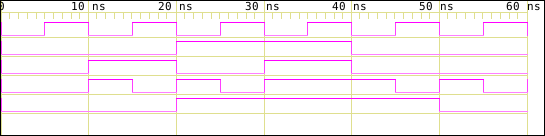
\includegraphics[width=\textwidth]{p1-proof}

As one can easily see:
 %
\begin{itemize}
    \item \texttt{x} mostly flips on every clock-change, except if \texttt{(a and b)}, as specified.
    \item \texttt{z} is the \texttt{or}'d output, with a delay of 10ns, as specified.
    \item there is no mystery.
\end{itemize}


\section*{Problem 2: VHDL 4-Bit Register}

see upload


\section*{Problem 3: Parking Lot}

see upload


\end{document}
